\documentclass[12pt,a4paper]{article}
\usepackage{lmodern}

\usepackage{placeins}
\usepackage{booktabs}
\usepackage{amssymb,amsmath}
\usepackage{ifxetex,ifluatex}
\usepackage{fixltx2e} % provides \textsubscript
\ifnum 0\ifxetex 1\fi\ifluatex 1\fi=0 % if pdftex
  \usepackage[T1]{fontenc}
  \usepackage[utf8]{inputenc}
\else % if luatex or xelatex
  \ifxetex
    \usepackage{mathspec}
    \usepackage{xltxtra,xunicode}
  \else
    \usepackage{fontspec}
  \fi
  \defaultfontfeatures{Mapping=tex-text,Scale=MatchLowercase}
  \newcommand{\euro}{€}
\fi
% use upquote if available, for straight quotes in verbatim environments
\IfFileExists{upquote.sty}{\usepackage{upquote}}{}
% use microtype if available
\IfFileExists{microtype.sty}{%
\usepackage{microtype}
\UseMicrotypeSet[protrusion]{basicmath} % disable protrusion for tt fonts
}{}
\usepackage[lmargin = 3 cm,rmargin = 2.5cm,tmargin=2.5cm,bmargin=2.5cm]{geometry}

% Figure Placement:
\usepackage{float}
\let\origfigure\figure
\let\endorigfigure\endfigure
\renewenvironment{figure}[1][2] {
    \expandafter\origfigure\expandafter[H]
} {
    \endorigfigure
}

%% citation setup
\usepackage{csquotes}

\usepackage[backend=biber, maxbibnames = 99, style = apa]{biblatex}
\setlength\bibitemsep{1.5\itemsep}
\addbibresource{R_packages.bib}
\bibliography{references.bib}
\usepackage{graphicx}
\makeatletter
\def\maxwidth{\ifdim\Gin@nat@width>\linewidth\linewidth\else\Gin@nat@width\fi}
\def\maxheight{\ifdim\Gin@nat@height>\textheight\textheight\else\Gin@nat@height\fi}
\makeatother
% Scale images if necessary, so that they will not overflow the page
% margins by default, and it is still possible to overwrite the defaults
% using explicit options in \includegraphics[width, height, ...]{}
\setkeys{Gin}{width=\maxwidth,height=\maxheight,keepaspectratio}
\ifxetex
  \usepackage[setpagesize=false, % page size defined by xetex
              unicode=false, % unicode breaks when used with xetex
              xetex]{hyperref}
\else
  \usepackage[unicode=true, linktocpage = TRUE]{hyperref}
\fi
\hypersetup{breaklinks=true,
            bookmarks=true,
            pdfauthor={Nils Paffen, David Schulze},
            pdftitle={Stay home and let the simulation play},
            colorlinks=true,
            citecolor=blue,
            urlcolor=blue,
            linkcolor=magenta,
            pdfborder={0 0 0}}
\urlstyle{same}  % don't use monospace font for urls
\setlength{\parindent}{0pt}
\setlength{\parskip}{6pt plus 2pt minus 1pt}
\setlength{\emergencystretch}{3em}  % prevent overfull lines
\setcounter{secnumdepth}{5}

%%% Use protect on footnotes to avoid problems with footnotes in titles
\let\rmarkdownfootnote\footnote%
\def\footnote{\protect\rmarkdownfootnote}

%%% Change title format to be more compact
\usepackage{titling}

% Create subtitle command for use in maketitle
\newcommand{\subtitle}[1]{
  \posttitle{
    \begin{center}\large#1\end{center}
    }
}

\setlength{\droptitle}{-2em}
  \title{Stay home and let the simulation play}
  \pretitle{\vspace{\droptitle}\centering\huge}
  \posttitle{\par}
\subtitle{Predicting regional football league outcomes with statistical methods}
  \author{Nils Paffen, David Schulze}
  \preauthor{\centering\large\emph}
  \postauthor{\par}
  \predate{\centering\large\emph}
  \postdate{\par}
  \date{today}

\usepackage{dcolumn, xcolor, amsmath}
\usepackage{booktabs}
\usepackage{longtable}
\usepackage{array}
\usepackage{multirow}
\usepackage{wrapfig}
\usepackage{float}
\usepackage{colortbl}
\usepackage{pdflscape}
\usepackage{tabu}
\usepackage{threeparttable}
\usepackage{threeparttablex}
\usepackage[normalem]{ulem}
\usepackage{makecell}

%% linespread settings

\usepackage{setspace}

\onehalfspacing

% Language Setup

\usepackage{ifthen}
\usepackage{iflang}
\usepackage[super]{nth}
\usepackage[ngerman, english]{babel}

%Acronyms
\usepackage[printonlyused, withpage, nohyperlinks]{acronym}
\usepackage{changepage}

% Multicols for the Title page
\usepackage{multicol}

\begin{document}

\selectlanguage{english}


%\maketitle

\begin{titlepage}
  \noindent\begin{minipage}{0.6\textwidth}
	  \IfLanguageName{english}{University of Duisburg-Essen}{Universität Duisburg-Essen}\\
	  \IfLanguageName{english}{Faculty of Business Administration and Economics}{Fakultät für Wirtschaftswissensschaften}\\
	  \IfLanguageName{english}{Chair of Economeics}{Lehrstuhl für Wirtschaftswissenschaften}\\
  \end{minipage}
	\begin{minipage}{0.4\textwidth}
	  \begin{flushright}
  	  \vspace{-0.5cm}
      \IfLanguageName{english}{\includegraphics*[width=5cm]{Includes/duelogo_en.png}}{\includegraphics*[width=5cm]{Includes/duelogo_de.png}}
	  \end{flushright}
	\end{minipage}
  \\
  \vspace{0.5cm}
  \begin{center}
  \huge{Stay home and let the simulation play}\\
  \vspace{.25cm}
  \Large{Predicting regional football league outcomes with statistical methods}\\
  \vspace{0.5cm}
  \large{Working Paper}\\
  \vspace{0.5cm}
  \large{  \IfLanguageName{english}{Submitted to the Faculty of \\ Economics  \\at the \\University of Duisburg-Essen}{Vorgelegt der \\Fakultät für Wirtschaftswissenschaften der \\ Universität Duisburg-Essen}\\}
  \vspace{0.75cm}
  \large{\IfLanguageName{english}{from:}{von:}}\\
  \vspace{0.5cm}
  Nils Paffen, David Schulze\\
  \end{center}
  %\vspace{2cm}
  \vfill
  \hrulefill

  \noindent\begin{minipage}[t]{0.3\textwidth}
  \IfLanguageName{english}{Reviewer:}{Erstgutachter:}
  \end{minipage}
  \begin{minipage}[t]{0.7\textwidth}
  \hspace{1cm}Prof.~Dr.~Christoph Hanck
  \end{minipage}

  \noindent\begin{minipage}[t]{0.3\textwidth}
  \IfLanguageName{english}{Deadline:}{Abgabefrist:}
  \end{minipage}
  \begin{minipage}[t]{0.7\textwidth}
  \hspace{1cm}
  \end{minipage}

  \hrulefill

  \begin{multicols}{3}

  Name:

  Matriculation Number:

  E-Mail:

  Study Path:

  Semester:

  Graduation (est.):
 
  \columnbreak

  David Schulze

  --
  
  david.schulze@rgs-econ.de

  PhD Economics

  \nth{2}

  -- 
  
  \columnbreak

  Nils Paffen

  3071594
  
  nils.paffen@stud.uni-due.de

  M.Sc. Economics

  \nth{2}

  Winter Term 2021

	\end{multicols}

\end{titlepage}

\newgeometry{top=2cm, left = 5cm, right = 2.5cm, bottom = 2.5cm}


\pagenumbering{Roman}
{
\hypersetup{linkcolor=black}

\setcounter{tocdepth}{3}
\tableofcontents
}

\newpage
\listoffigures
\addcontentsline{toc}{section}{List of Figures}

%\newpage
\listoftables
\addcontentsline{toc}{section}{List of Tables}

\section*{List of Abbreviations}
\addcontentsline{toc}{section}{List of Abbreviations}

\begin{adjustwidth}{1.5em}{0pt}

\begin{acronym}[dummyyyy]
 \acro{LASSO}{Least Absolute Shrinkage and Selection Operator}
 \acro{pcr}{Principal Components Regression}
 \acro{RMSE}{Root Mean Squared Error}
 \acro{MAE}{Mean Absolute Error}
 \acro{SEM}{Single Electricity Market}
 \acro{I-SEM}{Integrated Single Electricity Market}
 \acro{EU}{European Union}
 \acro{DM}{Diebold-Mariano}


%Falls eine Abkürzung in der Mehrzahl nicht einfach auf "s" endet muss das speziell eingestellt werden.
% \acro{slmtA}{super lange mega tolle Abkürzung} %Einzahl
 %\acroplural{slmtA}[slmtAs]{super lange mega tolle Abkürzungen} %Mehrzahl
 \acro{dummyyyy}{dummyyy}
\end{acronym}

\end{adjustwidth}

\restoregeometry

\newpage
\pagenumbering{arabic}
\hypertarget{abstract}{%
\section{Abstract}\label{abstract}}

Publicly available data and public attention are contributing to the
interest in forecasting football game results and the relevance of the
accuracy of those forecasts. Global pandemics like SARS-CoV2 are just
one reason why seasons may be canceled, providing a regular reason to
forecast missing games. We provide a short overview on the state of the
literature and use data from the aborted German local men's league
season 2019-20 to predict the season's outcome using three different
statistical approaches. A measure of each team's strength is calculated
from past games and used as quantifier in the simulation or prediction.
Instead of annulling the games played thus far or using the table as of
now, using a prediction algorithm to simulate that seasons end result
might be fairer. That's because the algorithm includes the played games
to make a better guess at the outcome of the missing games. Research has
shown that measures like the Elo rating system are better predictors of
a team's performance than for example current league table points on
their own. For this data set we find that gains from using advanced
methods are marginal when evaluating them with data from past seasons.
Methods are evaluated by calculating the correlation of the forecast
results for previous seasons with their actual outcomes.

\hypertarget{introduction}{%
\section{Introduction}\label{introduction}}

The Covid-19 epidemic forced sports leagues in Germany to suspend
championships that were already in full swing. For example, the local
men's league Recklinghausen class A1 finished around 150 games, before
all further matches were canceled starting from Sunday March 12, 2020,
leaving around 90 games left unplayed until the last planned day of the
league on Sunday May 24, 2020. It was very likely at the time that the
games could not be postponed to a later date, which turned out to be the
case. So it was natural for players and fans alike to ask the question:
\enquote{What would the outcome of the season have been?} We use data on
games already played from the website
\href{http://www.fussball.de/spieltagsuebersicht/re-kl-a-1-kreis-recklinghausen-kreisliga-a-herren-saison1920-westfalen/-/staffel/027II28DH8000009VS5489B3VS3GHJJU-G\#!/}{fussball.de}
to answer this question, drawing on established forecasting methods from
the literature.

The league system in Germany is structured so that everyone plays two
games against every opponent: The system colloquially known as
\enquote{Back and Forth} implies that each pair plays once at home and
once away in the other team's stadium. This means it's easier to
forecast than the tournament system of the World Cup. There in the group
stage, groups are determined by chance, a process known as
\enquote{seeding}. Groups then play a so-called round-robin tournament,
also known as all-play-all, were all group members play against each
other, which corresponds to the mode in which the German local leagues
play in each round. But the World Cup then continues with
single-elimination, or a knock-out stage, which introduces random path
dependencies that are not relevant for forecasting the Germany's local
leagues. This implies that the part of the existing literature on
forecasting results in the FIFA World Cup concerning the group stage
remains highly relevant for the task at hand, since the game rules are
otherwise identical.

In the next section, we give an overview of models used and evaluated
for the purpose of predicting football match outcomes in the past. We
introduce a small subset of models in more detail in the third part. The
fourth part contains the results from calculating a simulation based on
these for the local men's league Recklinghausen class A1. We also
present some comparative statistics of the model performance and draw
some conclusions in the last segment.

\hypertarget{literature}{%
\section{Literature}\label{literature}}

A natural starting point for the forecasting of match or season outcomes
in football tournaments is using the FIFA points ranking method that is
widely used to evaluate the strength of a team and updated after each
game. For example, a recent study by Correa et al.~\autocite*{correa}
uses FIFA points to forecast the results of the 2018 FIFA Men's World
Cup. This approach has however generated criticism
\textcite{mchale2007}, especially because it does not update based on
new information fast enough. The benchmark study by Lasek et
al.~\autocite*{lasek2013} compares established and proposed rankings.
They find that FIFA rankings perform slightly worse than alternative
methods, especially a version of the Elo rating system originally
proposed by Arpad Elo for the United States Chess Federation to rate
competitive chess players that was adapted for football championships by
the authors of the website EloRatings.net \autocite*{eloratings}.

Other studies show the effective prediction power of FIFA rankings,
e.g.~\textcite{suzuki2008}. Leitner et al.~\autocite*{leitner2010} find
that bookmakers odds are more predictive than FIFA rankings. In our case
we don't expect betting markets to be active enough to make this a
feasible approach, although it would be an interesting reference point.
We do however adopt their use of Spearman's rank correlation between
simulated and real final tournament rankings to evaluate models'
performance and complement it with Kendall's tau. Lasek et
al.~\autocite*{lasek2013} evaluate using rating points, which are less
relevant for our use case than the absolute rankings, which determine
whether a team advances, stays or drops out of a league.

We consider three models for our calculation: First, a benchmark model
based on the table points of each team at the time when the league was
aborted. Second, an Elo rating system, and third a simple model based on
the Poisson distribution.

The benchmark model calculates the probability of winning a match by
dividing a team's current points (victories are 3, draws are 2) by the
total of their and their opponent's points, we can call this the
\enquote{points model}. This model does not include the possibility of a
draw. The probability is not updated after each simulated game, because
this does not generate new information about a team's strength.
Averaging the results over enough simulations, this approach will
converge to the current table ranking, so it is in fact just a weighted
randomization of the current table.

The second model is based on a version of the Elo rating system
published anonymously on the website EloRatings.net
\autocite*{eloratings}. The algorithm was originally developed for
ranking chess players. As an \enquote{earned} rating system
(\textcite{lasek2013}) a team's rating is updated iteratively according
to the outcome of single matches and depending on the expected outcome
with regard to the opponent's rating. This version was especially
adapted for the use in ranking football teams. Glickman
\autocite*{glickman1995} offers a comprehensive discussion of the Elo
rating system. ELO RATING DRAW???

The third model is a regression model that approximates the distribution
of goals in each game to a Poisson or Negative Binomial distribution
with an estimated constant parameter to adjust for the home advantage.
This approach follows the literature influenced by \textcite{maher1982}
and others. Generally, these models include different parameters to
allow for team-specific strengths when playing home or away, and while
defending or attacking. Other parameters to include random effects, for
example, can be added. We omit them here for simplicity. For a general
discussion see \textcite{karlis2003}. Many extensions of this model as
well as model selection algorithms are possible.

For a more recent review of advances in the literature and a new
approach based on the Weinbull distribution we refer to
\textcite{boshnakov2017}. They use an evaluation based on calibration
curves as well as the payoff from betting strategies and find that their
model improves on previous models and can yield positive betting
returns.

\hypertarget{data}{%
\section{Data}\label{data}}

For our simulation study we decided to use data from the local men's
league Recklinghausen class A1 in Westphalia for the 2019/2020 season.
16 clubs were scheduled to play against each other on a total of 30
match days in one home and one away game each. Due to the SARS-CoV2
pandemic, the association has decided to cancel all matches from March
15, 2020. 20 match days have already been played up to this point in
time which corresponds to a database of 158 matches. As the first half
of the season had already been completed, each team had already played
at least once against each team in the league. The extraction of real
data from websites using scraping scripts can be complicated, as website
operators have an interest in protecting their data from such automated
queries. \enquote{Fussball.de} is a website of the DFB (German Football
Association) which acts as a collection point for match results and
news, especially in the amateur sector. In its
\href{http://www.fussball.de/terms.and.conditions\#!/}{terms and
conditions page}, the DFB GmbH restricts the permanent storage of
content from the website and commercial use. Therefore we can't store
and or share the original data, but only the code we used to create them
and the results that we derived from them.

The game results cannot be extracted directly from the website. They are
masked, so they are made unreadable when viewing the HTML file and are
only evaluated afterwards using javascript and transferred to the CSS of
the site. The site also offers a match report, which graphically
represents a temporal course of the match. This is broken down in the
HTML code, in contrast to the match results, unmasked, and shows the
course of the match in text form. With the help of regular expression
operations, the game result can be reconstructed. The data record was
then divided into completed and missing games. The latter amount to 89
in this season, which were simulated with the methods described in the
following sections.

Table 1 shows the results after the 20th match day of the local men's
league Recklinghausen class A1 in Westphalia for the 2019/2020 season.
The column \emph{Goal Diff.} describes how many goals a team scored
subtracted by the amount of goals scored against them. Both numbers can
be extracted from the former column \emph{Goal Relation}, where the
first number describes the amount of scored goals of a team. The club
\enquote{VfL Ramsdorf} is leading the league with 52 Points and a goal
difference of 53. Followed by \enquote{TuS Gahlen} which is 6 points
short in the competition for the league's first place. The other end of
the table shows the club \enquote{SV Altendorf Ulfkotte} on the last
place with only 7 points and a goal difference of -84. It is preceded by
\enquote{Adler Weske II} which achieved 10 points and secured position
15 with a goal difference of -41. Especially the two first and the two
last positions in most football leagues are of special interest since
those teams could be promoted from the present league called
\enquote{Kreisliga} to the next higher league called
\enquote{Bezirksliga} or relegated to the lower league called
\enquote{Kreisliga B}. Given these results, we expected a high chance
for the club \enquote{VfL Ramsdorf} to secure a promotion spot while we
expected a fight against relegation between \enquote{TuS 05 Sinsen II},
\enquote{Adler Weske II} and \enquote{SV Altendorf-Ulfkotte}.

\begin{table}[H]

\caption{\label{tab:unnamed-chunk-1}Results after Matchday 20 Season 19/20}
\centering
\resizebox{\linewidth}{!}{
\begin{tabular}[t]{rllrrrlrr}
\toprule
Rank & Club & Games & Wins & Ties & Loss & Goal Relation & Goal Diff. & Points\\
\midrule
\cellcolor{gray!6}{1} & \cellcolor{gray!6}{VfL Ramsdorf} & \cellcolor{gray!6}{20} & \cellcolor{gray!6}{17} & \cellcolor{gray!6}{1} & \cellcolor{gray!6}{2} & \cellcolor{gray!6}{74 : 21} & \cellcolor{gray!6}{53} & \cellcolor{gray!6}{52}\\
2 & TuS Gahlen & 20 & 14 & 4 & 2 & 54 : 15 & 39 & 46\\
\cellcolor{gray!6}{3} & \cellcolor{gray!6}{SV Schermbeck II} & \cellcolor{gray!6}{20} & \cellcolor{gray!6}{14} & \cellcolor{gray!6}{3} & \cellcolor{gray!6}{3} & \cellcolor{gray!6}{60 : 24} & \cellcolor{gray!6}{36} & \cellcolor{gray!6}{45}\\
4 & Fenerbahce I. Marl & 20 & 13 & 2 & 5 & 41 : 36 & 5 & 41\\
\cellcolor{gray!6}{5} & \cellcolor{gray!6}{TSV Raesfeld} & \cellcolor{gray!6}{20} & \cellcolor{gray!6}{12} & \cellcolor{gray!6}{2} & \cellcolor{gray!6}{6} & \cellcolor{gray!6}{72 : 29} & \cellcolor{gray!6}{43} & \cellcolor{gray!6}{38}\\
\addlinespace
6 & 1. SC BW Wulfen & 19 & 12 & 1 & 6 & 58 : 32 & 26 & 37\\
\cellcolor{gray!6}{7} & \cellcolor{gray!6}{TuS Velen} & \cellcolor{gray!6}{20} & \cellcolor{gray!6}{9} & \cellcolor{gray!6}{2} & \cellcolor{gray!6}{9} & \cellcolor{gray!6}{44 : 44} & \cellcolor{gray!6}{0} & \cellcolor{gray!6}{29}\\
8 & SC Marl-Hamm & 19 & 9 & 0 & 10 & 53 : 52 & 1 & 27\\
\cellcolor{gray!6}{9} & \cellcolor{gray!6}{SV Lembeck} & \cellcolor{gray!6}{20} & \cellcolor{gray!6}{8} & \cellcolor{gray!6}{3} & \cellcolor{gray!6}{9} & \cellcolor{gray!6}{49 : 48} & \cellcolor{gray!6}{1} & \cellcolor{gray!6}{27}\\
10 & BVH Dorsten & 19 & 8 & 2 & 9 & 46 : 33 & 13 & 26\\
\addlinespace
\cellcolor{gray!6}{11} & \cellcolor{gray!6}{FC RW Dorsten} & \cellcolor{gray!6}{20} & \cellcolor{gray!6}{6} & \cellcolor{gray!6}{5} & \cellcolor{gray!6}{9} & \cellcolor{gray!6}{28 : 41} & \cellcolor{gray!6}{-13} & \cellcolor{gray!6}{23}\\
12 & Westfalia Gemen II & 20 & 6 & 2 & 12 & 38 : 60 & -22 & 20\\
\cellcolor{gray!6}{13} & \cellcolor{gray!6}{SC Reken II} & \cellcolor{gray!6}{19} & \cellcolor{gray!6}{4} & \cellcolor{gray!6}{3} & \cellcolor{gray!6}{12} & \cellcolor{gray!6}{41 : 61} & \cellcolor{gray!6}{-20} & \cellcolor{gray!6}{15}\\
14 & TuS 05 Sinsen II & 20 & 2 & 5 & 13 & 25 : 62 & -37 & 11\\
\cellcolor{gray!6}{15} & \cellcolor{gray!6}{Adler Weseke II} & \cellcolor{gray!6}{20} & \cellcolor{gray!6}{2} & \cellcolor{gray!6}{4} & \cellcolor{gray!6}{14} & \cellcolor{gray!6}{23 : 64} & \cellcolor{gray!6}{-41} & \cellcolor{gray!6}{10}\\
\addlinespace
16 & SV Altendorf-Ulfkotte & 20 & 2 & 1 & 17 & 17 : 101 & -84 & 7\\
\bottomrule
\end{tabular}}
\end{table}

For further analysis we decided to scrape the data of season 16/17,
17/18 and 18/19, so we could perform out-of-sample error (OOSE) test
statistics. The latter will indicate the predictive performance of the
different methods.

\hypertarget{predictive-models}{%
\section{Predictive Models}\label{predictive-models}}

To predict the outcome of the canceled games, we determine each team's
relative strength using each of the three candidate models. Based on
this we simulate or predict the end of the 2019/2020 season by
calculating a winning probability for each missing game. Specifically we
implement

\begin{itemize}
\item the points model,
\item the EloRankings.net model, 
\item a Poisson/Negative Binomial regression model
\end{itemize}

The first model is just a simple baseline model that calculates the
probability of a team \emph{A} winning a game against team \emph{B}
using the formula

\begin{align}
P(\text{\emph{A wins}}) = \frac{table points_A}{{table points}_A + {table points}_B},
\end{align}

where \emph{tablepoints} corresponds to the number of games won at the
current state of the season (valued at three points) plus the number of
draws (valued at one point). This value also governs the ranking and
ultimate placement of the teams in the league. Two issues arise from
this approach. Firstly, should the probability based on table points be
updated after each simulated game? We argue no, because this would not
include new information about the relative strength of the teams and
just increase the variance of the result.

Secondly, the average over many simulated runs will converge to the
initial table from when the season was interrupted. This will defeat the
purpose of running a simulation in the first place, because it does not
yield any new information, and we could have just used the table as it
was. In case a random draw is used to determine the result, this method
is however preferable to an unweighted coin toss, because that would
unfairly favor below-average teams.

Our second model is based on the rating algorithm from
\href{eloratings.net/about}{eloratings.net}. The anonymous site operator
uses the following formulation of the rating. Here, the new rating
\(R_n\) is defined as an update of \(R_0\), which is the old rating. The
rating is updated, if the outcome differs from what the old rating
predicted. The size of the update, or the learning speed of the
algorithm, is moderated according to the importance of the match and the
goal difference.

\begin{align}
R_n = R_0 + K * (W - W_e) &
\end{align}

\begin{align}
K = \begin{cases}
    K_0         &\mbox{if won by 1 goal} \\
    K_0 * 1.5   &\mbox{if won by 2 goals} \\
    K_0 * 0.75  &\mbox{if won by 3 goals} \\
    K_0 * \left( 0.75 + K_0 * \frac{N-3}{8} \right) &\mbox{if won by 4 or more goals})
  \end{cases}
\end{align}

The weighting factor \emph{K} for each match is based on \(K_0\), the
type of tournament in which the match takes place. The values range from
World Cup finals (60) to friendly matches (20). Regular tournament
matches are given a weighting factor of 30, which we also use here.
\(K_0\) is then adjusted for the goal difference of the game outcome
(how significant a victory or loss was) according to the formula above.
A higher goal difference will have a higher impact on the final rating.
\emph{W} is the result of the match: 0 for a loss, 0.5 for a draw and 1
for a win. \(W_e\) is the probability of winning defined by the
following formula:

\begin{align}
W_e = \frac{1}{/(10^{(-dr/400)}+1),}
\end{align}

where \emph{dr} is defined as the rating difference and the home team
receives an arbitrary bonus of 100 points. This bonus is considered to
be a psychological advantage resulting from the fact that the game is
played on the home pitch (see, e.g., \textcite{Pollard2008}).

To simulate the outcome of the league with the points and Elo ranking
method, we follow Correa et al.~\autocite*{correa} and draw the results
of each game from a Bernoulli distribution with the parameter \emph{p}
equal to the winning probability obtained from each method.

To account for draws when simulating the outcome with the Elo method, we
use the share of draws in the current season as the likelihood of a
draw. Half of this is deducted from the home team's winning probability
and half from the away team's winning probability. If this puts any
probability into negative, this amount is then added to the opposite
probability. Then the game result is drawn from this distribution. We
repeated this procedure for all games and evaluated the results with 3
points for the winning team, 1 point for both teams in case of a draw
and 0 points for the losing team.

Our third model uses regressions based on the Poisson and negative
binomial distributions to predict match outcomes as the number of goals
scored in each match. The probability matrix from which the game result
is drawn is a \(n \times n\) matrix where each cell indicates the
probability of that specific match result. While the rows indicates the
goals of the home team, the column indicates the goals of the away team.
For example the cell of the first row and in the first column indicates
the likelihood that both teams score \(0\) goals. The maximum number of
goals \emph{n} can be set high enough to cover the range of possible
outcomes. Because the highest number of goals scored since 2016 in any
one game was 14, we set \emph{n} equal to 15. The Poisson probability
mass function of our model can be expressed as:

\begin{align}
P(x) = \dfrac{e^{-\lambda}\lambda^x}{x!}, \lambda > 0
\end{align}

where \(\lambda\) represents the average number of goals. First, we
estimate a log-linear Poisson regression model using data from the
matches already played:

\begin{align}
log(\text{\emph{goals by team}}) \sim constant + \beta_1 home + \sum_{i}^{T} \beta_i team + \sum_{j}^{T} \beta_j opponent
\end{align}

Here \emph{goals by team} represents the number of goals scored by the
team in a certain game. The dummy variable \emph{home} equals 1 if the
team plays on it's home pitch, and \emph{team} and \emph{opponent}
represent dummies for each team out of a total of \emph{T} teams
respectively. So each game is represented twice: Once from the defending
home team and once from the opponents view. Because it is a model in
log-transformation, the exponential of the parameters \(\beta_i\) and
\(\beta_j\) then represent the change in expected number of goals scored
by the home team. The exponential of the constant specifies the overall
expected value of goals if a team plays away, and \(e^{\beta_1}\) is the
expected effect of the home field advantage. This could be seen as an
improvement over the Elo model, because we do not fix this effect in
advance.

To estimate the model, we use the \emph{glm} function from the R
\emph{stats} package. With the option \emph{family =
quasipoisson(link=log)}, a Quasi-Maximum Likelihood Estimation of the
log-transformation is calculated. The reason for choosing a
Quasi-Poisson distribution is that this adjusts the standard-errors for
overdispersion (the variance is larger than the mean). The resulting
predictions do not change if one instead uses the standard Poisson
distribution. A test from the \emph{AER} package finds low significance
for overdispersion (estimate: 1.13, z = 1.5215, p-value = 0.064).
Pearson's Chi-Squared goodness-of-fit test finds that the model does not
fit the data very well (p = 0.00) The residual deviance (388.56) using
the Poisson distribution is much larger than the degrees of freedom
(284), so we estimate the model with a negative binomial distribution.
We follow the method proposed in Cameron and Trivedi
\autocite*{cameron2013}.

\begin{table}[!htbp] \centering 
  \caption{19/20 Season Regression Output for the Negative Binomial Model} 
  \label{} 
\small 
\begin{tabular}{@{\extracolsep{-50pt}}lD{.}{.}{-3} D{.}{.}{-3} D{.}{.}{-3} } 
\\[-1.8ex]\hline 
\hline \\[-1.8ex] 
\\[-1.8ex] & \multicolumn{3}{c}{goals} \\ 
 & \multicolumn{1}{c}{control} & \multicolumn{1}{c}{team} & \multicolumn{1}{c}{opponent} \\ 
\\[-1.8ex] & \multicolumn{1}{c}{(1)} & \multicolumn{1}{c}{(2)} & \multicolumn{1}{c}{(3)}\\ 
\hline \\[-1.8ex] 
 Constant & 0.762^{***}$ $(0.241) &  &  \\ 
  homey & 0.250^{***}$ $(0.081) &  &  \\ 
  Adler Weseke II &  & -1.065^{***}$ $(0.261) & 0.606^{***}$ $(0.230) \\ 
  BVH Dorsten &  & -0.314$ $(0.214) & 0.049$ $(0.262) \\ 
  FC RW Dorsten &  & -0.877^{***}$ $(0.243) & 0.181$ $(0.248) \\ 
  Fenerbahce I. Marl &  & -0.568^{***}$ $(0.219) & 0.098$ $(0.256) \\ 
  SC Marl-Hamm &  & -0.155$ $(0.206) & 0.500^{**}$ $(0.239) \\ 
  SC Reken II &  & -0.420^{*}$ $(0.220) & 0.691^{***}$ $(0.233) \\ 
  SV Altendorf-Ulfkotte &  & -1.272^{***}$ $(0.288) & 1.088^{***}$ $(0.218) \\ 
  SV Lembeck &  & -0.234$ $(0.210) & 0.354$ $(0.242) \\ 
  SV Schermbeck II &  & -0.180$ $(0.201) & -0.262$ $(0.281) \\ 
  TSV Raesfeld &  & 0.007$ $(0.194) & -0.090$ $(0.269) \\ 
  TuS 05 Sinsen II &  & -0.910^{***}$ $(0.252) & 0.589^{**}$ $(0.231) \\ 
  TuS Gahlen &  & -0.288$ $(0.206) & -0.814^{**}$ $(0.324) \\ 
  TuS Velen &  & -0.428^{**}$ $(0.216) & 0.276$ $(0.245) \\ 
  VfL Ramsdorf &  & 0.062$ $(0.192) & -0.445$ $(0.293) \\ 
  Westfalia Gemen II &  & -0.574^{**}$ $(0.223) & 0.593^{**}$ $(0.233) \\ 
 Observations & \multicolumn{1}{c}{316} & \multicolumn{1}{c}{316} & \multicolumn{1}{c}{316} \\ 
R$^{2}$ & \multicolumn{1}{c}{0.165} & \multicolumn{1}{c}{0.165} & \multicolumn{1}{c}{0.165} \\ 
Adjusted R$^{2}$ & \multicolumn{1}{c}{0.121} & \multicolumn{1}{c}{0.121} & \multicolumn{1}{c}{0.121} \\ 
Residual Std. Error (df = 299) & \multicolumn{1}{c}{1.967} & \multicolumn{1}{c}{1.967} & \multicolumn{1}{c}{1.967} \\ 
F Statistic (df = 16; 299) & \multicolumn{1}{c}{3.704$^{***}$} & \multicolumn{1}{c}{3.704$^{***}$} & \multicolumn{1}{c}{3.704$^{***}$} \\ 
\hline \\[-1.8ex] 
\textit{Notes:} & \multicolumn{3}{l}{$^{***}$Significant at the 1 percent level.} \\ 
 & \multicolumn{3}{l}{$^{**}$Significant at the 5 percent level.} \\ 
 & \multicolumn{3}{l}{$^{*}$Significant at the 10 percent level.} \\ 
\end{tabular} 
\end{table}

Note here that \enquote{1. SC BW Wulfen} is chosen as the base and no
dummy for it is included to avoid perfect multicollinearity. Its
parameter is set to zero and all other parameters can be seen as the
deviation from it. Also, for season 16/17 the team \enquote{VfB Hüls II
zg.} forfeit before the season started. Therefore all games were
canceled and the team was assigned to the last place of the seasons
table (place 18).

In summary, the coefficients of the model show that the club
\enquote{Altendorf-Ulfkotte}, is least likely to score a goal (low team
estimate) and teams playing against them have the highest chance to
score (high opponent estimate), with both estimates being highly
significant. Since the club is in the last place in the current table,
as mentioned in the data section, this is the expected result.
Conversely, we observe the something like the opposite for the current
table leader \enquote{VfL Ramsdorf}. For the simulation the result is
drawn from the negative binomial and Poisson distributions, and the
score probabilities are based on the estimated parameters.

The results from the estimation with a Poisson distribution are very
similar. However, the residual difference is higher (388.56 compared to
354.50), indicating a better fit. The goodness-of-fit test still rejects
the model (p = 0.00). The estimation results for Poisson can be found in
the Appendix.

Instead of simulating the result as with the first two methods, we can
simply calculate the expected number of goals based on the regression
estimate and sum up the expected final league table.

We can evaluate the fit of the distributions also by looking at
histograms comparing the actual distributions in the seasons before
against the model's predictions. For this purpose we pool the values of
all away and home goals of one season. As can be seen in the example
plot for season 16/17, the model does not predict enough outliers of
high goal numbers and predicts too many one- and two-goal outcomes. This
is representative for all three preceding seasons, as can be seen by the
other plots in the Appendix. This opens up the possibility of using a
different distribution, which is not pursued further in this paper.

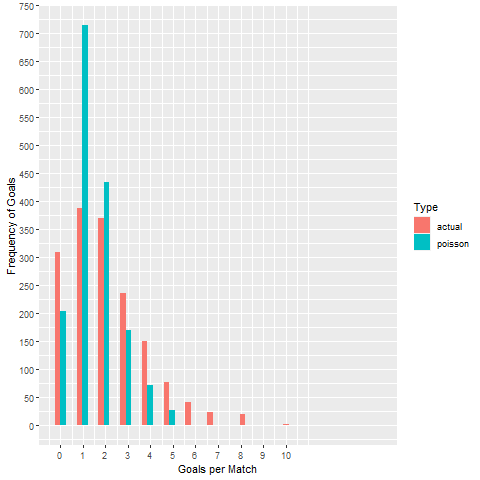
\includegraphics[width=12.11in]{C:/Users/Nils/Documents/GitHub/Fussball.de-Vorhersage/paper/plots/poisson_actual_home_1617}

A few alternatives have been developed for forecasting football games.
The potential of using independent Poisson distributions to match the
empirical distribution of goals scored by a team has been improved by
introducing correlation between the teams playing against one another in
a bivariate Poisson distribution \textcite{karlis2003}.

Boshnakov et al.~\autocite*{boshnakov2016} use a Weibull count model to
improve on the bivariate Poisson model, allowing them even to outperform
betting market in selected bets. Further analysis could compare the
predictive performance of models based on other distributions as well.

\hypertarget{results}{%
\section{Results}\label{results}}

Simulation for the Elo model was repeated until the rate of change of
the point average was 1\% or less. Aggregation to this point occurred
after about 2580 runs.

Looking at the final predictions for the 19/20 season, a few
observations stand out. First and foremost, the two relegation spots at
the top and bottom end of the table stay the same in each simulation. In
the middle field however, the models disagree and rate the teams there
very close to each other. The points and Elo method predict more
similarly, as well as (Quasi-)Poisson and the negative binomial model.
The last two are almost identical. Only TuS Velen gains an extra point
in (Quasi-)Poisson, which doesn't affect the ranking. Quasi- and
standard Poisson results are identical.

\begin{table}[H]

\caption{\label{tab:unnamed-chunk-6}Simulated Final Score Table}
\centering
\resizebox{\linewidth}{!}{
\begin{tabular}[t]{rlrlrlrlr}
\toprule
\multicolumn{1}{c}{ } & \multicolumn{2}{c}{Points Model} & \multicolumn{2}{c}{Elo Rating Model} & \multicolumn{2}{c}{(Quasi-)Poisson Model} & \multicolumn{2}{c}{Neg.Binomial Model} \\
\cmidrule(l{3pt}r{3pt}){2-3} \cmidrule(l{3pt}r{3pt}){4-5} \cmidrule(l{3pt}r{3pt}){6-7} \cmidrule(l{3pt}r{3pt}){8-9}
rank & club\_pnt & score\_pnt & club\_e & score\_e & club\_psn & score\_psn & club\_nbin & score\_nbin\\
\midrule
\cellcolor{gray!6}{1} & \cellcolor{gray!6}{VfL Ramsdorf} & \cellcolor{gray!6}{72.20} & \cellcolor{gray!6}{VfL Ramsdorf} & \cellcolor{gray!6}{64.35} & \cellcolor{gray!6}{VfL Ramsdorf} & \cellcolor{gray!6}{80} & \cellcolor{gray!6}{VfL Ramsdorf} & \cellcolor{gray!6}{80}\\
2 & TuS Gahlen & 65.04 & TuS Gahlen & 58.74 & TuS Gahlen & 72 & TuS Gahlen & 72\\
\cellcolor{gray!6}{3} & \cellcolor{gray!6}{SV Schermbeck II} & \cellcolor{gray!6}{63.51} & \cellcolor{gray!6}{SV Schermbeck II} & \cellcolor{gray!6}{57.74} & \cellcolor{gray!6}{1. SC BW Wulfen} & \cellcolor{gray!6}{67} & \cellcolor{gray!6}{1. SC BW Wulfen} & \cellcolor{gray!6}{67}\\
4 & Fenerbahce I. Marl & 58.06 & Fenerbahce I. Marl & 53.52 & SV Schermbeck II & 65 & SV Schermbeck II & 65\\
\cellcolor{gray!6}{5} & \cellcolor{gray!6}{1. SC BW Wulfen} & \cellcolor{gray!6}{57.22} & \cellcolor{gray!6}{1. SC BW Wulfen} & \cellcolor{gray!6}{50.88} & \cellcolor{gray!6}{TSV Raesfeld} & \cellcolor{gray!6}{62} & \cellcolor{gray!6}{TSV Raesfeld} & \cellcolor{gray!6}{62}\\
\addlinespace
6 & TSV Raesfeld & 55.75 & TSV Raesfeld & 50.64 & Fenerbahce I. Marl & 50 & Fenerbahce I. Marl & 50\\
\cellcolor{gray!6}{7} & \cellcolor{gray!6}{TuS Velen} & \cellcolor{gray!6}{45.38} & \cellcolor{gray!6}{TuS Velen} & \cellcolor{gray!6}{41.79} & \cellcolor{gray!6}{SV Lembeck} & \cellcolor{gray!6}{46} & \cellcolor{gray!6}{SV Lembeck} & \cellcolor{gray!6}{48}\\
8 & SV Lembeck & 44.15 & SC Marl-Hamm & 40.91 & BVH Dorsten & 44 & BVH Dorsten & 44\\
\cellcolor{gray!6}{9} & \cellcolor{gray!6}{SC Marl-Hamm} & \cellcolor{gray!6}{43.88} & \cellcolor{gray!6}{BVH Dorsten} & \cellcolor{gray!6}{39.90} & \cellcolor{gray!6}{SC Marl-Hamm} & \cellcolor{gray!6}{44} & \cellcolor{gray!6}{SC Marl-Hamm} & \cellcolor{gray!6}{44}\\
10 & BVH Dorsten & 42.64 & SV Lembeck & 39.57 & TuS Velen & 41 & TuS Velen & 40\\
\addlinespace
\cellcolor{gray!6}{11} & \cellcolor{gray!6}{FC RW Dorsten} & \cellcolor{gray!6}{37.59} & \cellcolor{gray!6}{FC RW Dorsten} & \cellcolor{gray!6}{35.82} & \cellcolor{gray!6}{FC RW Dorsten} & \cellcolor{gray!6}{28} & \cellcolor{gray!6}{FC RW Dorsten} & \cellcolor{gray!6}{28}\\
12 & Westfalia Gemen II & 32.82 & Westfalia Gemen II & 32.40 & Westfalia Gemen II & 27 & Westfalia Gemen II & 27\\
\cellcolor{gray!6}{13} & \cellcolor{gray!6}{SC Reken II} & \cellcolor{gray!6}{27.60} & \cellcolor{gray!6}{SC Reken II} & \cellcolor{gray!6}{29.11} & \cellcolor{gray!6}{SC Reken II} & \cellcolor{gray!6}{25} & \cellcolor{gray!6}{SC Reken II} & \cellcolor{gray!6}{25}\\
14 & TuS 05 Sinsen II & 21.28 & TuS 05 Sinsen II & 23.86 & TuS 05 Sinsen II & 15 & TuS 05 Sinsen II & 15\\
\cellcolor{gray!6}{15} & \cellcolor{gray!6}{Adler Weseke II} & \cellcolor{gray!6}{18.88} & \cellcolor{gray!6}{Adler Weseke II} & \cellcolor{gray!6}{22.60} & \cellcolor{gray!6}{Adler Weseke II} & \cellcolor{gray!6}{15} & \cellcolor{gray!6}{Adler Weseke II} & \cellcolor{gray!6}{15}\\
\addlinespace
16 & SV Altendorf-Ulfkotte & 13.98 & SV Altendorf-Ulfkotte & 19.50 & SV Altendorf-Ulfkotte & 7 & SV Altendorf-Ulfkotte & 7\\
\bottomrule
\end{tabular}}
\end{table}

\begin{verbatim}
## `stat_bin()` using `bins = 30`. Pick better value with `binwidth`.
\end{verbatim}

\begin{verbatim}
## `stat_bin()` using `bins = 30`. Pick better value with `binwidth`.
\end{verbatim}

\hypertarget{oose-test-statistics}{%
\section{OOSE Test Statistics}\label{oose-test-statistics}}

Making predictions of events that might never happen can obviously be
criticized with a simple question. How do you know that your results
reflect reality as good as possible? Following George E. P. Box who is
known for his quote \enquote{All models are wrong}, which is often
amended by \enquote{but some are useful}, we want to show that our
models cover the latter. The out-of-sample error test statistic is one
way to achieve this. One simply divides a data set into a small test
data set and a larger training data set. For the seasons of 16/17, 17/18
and 18/19, we split the data sets after the number of games, after which
the SARS-Cov2 pandemic forced the 19/20 season to abort. This way we
increase the relevance for our use case.

Following \textcite{leitner2010}, we evaluate the models' performance
using the rank correlation between their predicted and the real ranking
tables for the three past years' seasons (2016, 2017 and 2018). We show
both Kendall's tau and Spearman's rho rank correlation coefficients.
Generally, no model performs best in all seasons. The Elo method however
performs generally better than the regression models' predictions.
Surprisingly, the benchmark points method performs best in two out of
three seasons.

Because no model is cleafrly better then the others, and performance
varies a lot between seasons, we see no clear evidence that one method
should be preferred. A simulation based on these predictions would
however be much fairer than a coin toss.

\begin{table}[ht]
\centering
\begin{tabular}{lrr}
  \hline
method & spearmans\_rho & kendalls\_tau \\ 
  \hline
elo ranking & 0.98 & 0.93 \\ 
  nbinom & 0.96 & 0.86 \\ 
  points & 0.98 & 0.94 \\ 
  poisson & 0.96 & 0.89 \\ 
  quasipoisson & 0.96 & 0.89 \\ 
   \hline
\end{tabular}
\caption{Average rank correlation coefficients for simulation and actual data} 
\end{table} 


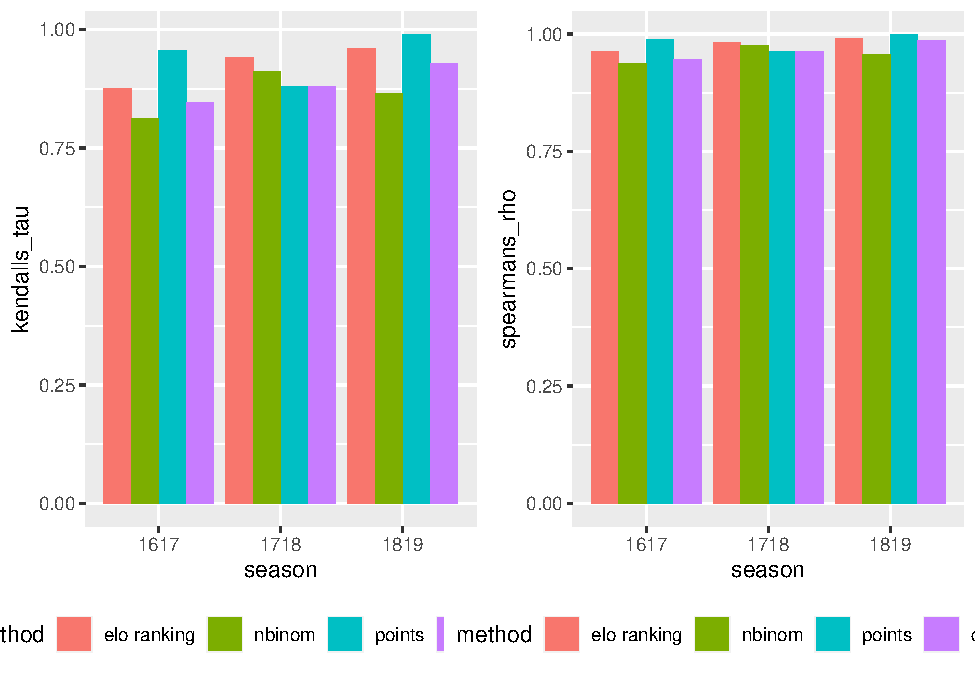
\includegraphics{term_paper_eem_files/figure-latex/unnamed-chunk-9-1.pdf}

\hypertarget{conclusion}{%
\section{Conclusion}\label{conclusion}}

The decision to quit all games later than 8th of March because of the
pandemic was not revised while the infection rates relaxed during May
and June in Germany. Combined with the unforeseeable future of the
SARS-Cov2 pandemic, a more fair and balanced decision making process
could include statistical learning techniques, such as those shown in
this paper.

We find that neither a simulation using a weighted coin toss based on
the current league table (the points method), one based on the Elo
ranking, or one based on regressions using (Quasi-)Poisson or negative
binomial methods is superior. Therefore we cannot recommend one in
particular.

\newpage

\printbibliography

\newpage

\hypertarget{appendix}{%
\section{Appendix}\label{appendix}}

\begin{table}[!htbp] \centering 
  \caption{19/20 Season Regression Output for the Quasi-Poisson Model} 
  \label{} 
\small 
\begin{tabular}{@{\extracolsep{-30pt}}lD{.}{.}{-3} D{.}{.}{-3} D{.}{.}{-3} } 
\\[-1.8ex]\hline 
\hline \\[-1.8ex] 
\\[-1.8ex] & \multicolumn{3}{c}{goals} \\ 
 & \multicolumn{1}{c}{control} & \multicolumn{1}{c}{team} & \multicolumn{1}{c}{opponent} \\ 
\\[-1.8ex] & \multicolumn{1}{c}{(1)} & \multicolumn{1}{c}{(2)} & \multicolumn{1}{c}{(3)}\\ 
\hline \\[-1.8ex] 
 Constant & 0.752^{***}$ $(0.255) &  &  \\ 
  homey & 0.241^{***}$ $(0.085) &  &  \\ 
  Adler Weseke II &  & -1.047^{***}$ $(0.278) & 0.595^{**}$ $(0.244) \\ 
  BVH Dorsten &  & -0.289$ $(0.223) & 0.051$ $(0.280) \\ 
  FC RW Dorsten &  & -0.877^{***}$ $(0.259) & 0.178$ $(0.265) \\ 
  Fenerbahce I. Marl &  & -0.564^{**}$ $(0.230) & 0.109$ $(0.273) \\ 
  SC Marl-Hamm &  & -0.145$ $(0.214) & 0.507^{**}$ $(0.253) \\ 
  SC Reken II &  & -0.405^{*}$ $(0.230) & 0.697^{***}$ $(0.246) \\ 
  SV Altendorf-Ulfkotte &  & -1.252^{***}$ $(0.310) & 1.089^{***}$ $(0.229) \\ 
  SV Lembeck &  & -0.216$ $(0.219) & 0.356$ $(0.257) \\ 
  SV Schermbeck II &  & -0.167$ $(0.208) & -0.267$ $(0.304) \\ 
  TSV Raesfeld &  & 0.021$ $(0.200) & -0.085$ $(0.288) \\ 
  TuS 05 Sinsen II &  & -0.902^{***}$ $(0.269) & 0.581^{**}$ $(0.244) \\ 
  TuS Gahlen &  & -0.266$ $(0.214) & -0.812^{**}$ $(0.352) \\ 
  TuS Velen &  & -0.409^{*}$ $(0.225) & 0.280$ $(0.261) \\ 
  VfL Ramsdorf &  & 0.072$ $(0.198) & -0.435$ $(0.316) \\ 
  Westfalia Gemen II &  & -0.559^{**}$ $(0.235) & 0.591^{**}$ $(0.246) \\ 
 \hline \\[-1.8ex] 
\textit{Notes:} & \multicolumn{3}{l}{$^{***}$Significant at the 1 percent level.} \\ 
 & \multicolumn{3}{l}{$^{**}$Significant at the 5 percent level.} \\ 
 & \multicolumn{3}{l}{$^{*}$Significant at the 10 percent level.} \\ 
\end{tabular} 
\end{table}

% latex table generated in R 4.0.0 by xtable 1.8-4 package
% Fri Aug 28 12:11:16 2020
\begin{table}[ht]
\centering
\begin{tabular}{llrr}
  \hline
method & season & spearmans\_rho & kendalls\_tau \\ 
  \hline
elo ranking & 1617 & 0.96 & 0.88 \\ 
  elo ranking & 1718 & 0.98 & 0.94 \\ 
  elo ranking & 1819 & 0.99 & 0.96 \\ 
  points & 1617 & 0.97 & 0.90 \\ 
  points & 1718 & 0.96 & 0.88 \\ 
  points & 1819 & 1.00 & 0.97 \\ 
  poisson & 1617 & 0.94 & 0.85 \\ 
  poisson & 1718 & 0.96 & 0.88 \\ 
  poisson & 1819 & 0.99 & 0.93 \\ 
   \hline
\end{tabular}
\caption{Rank correlation coefficients for simulation and actual data} 
\end{table} 




\end{document}
